\documentclass[11pt,a4paper]{article}
\usepackage[utf8]{inputenc}
\usepackage[portuguese]{babel}
\usepackage[T1]{fontenc}
\usepackage[left=1.7cm,right=1.5cm,top=2.5cm,bottom=2cm]{geometry}
\usepackage{xcolor}
\definecolor{orange}{RGB}{255,127,0}
%\usepackage[dvipsnames]{xcolor}
\usepackage{titlesec}
\usepackage[utf8]{inputenc}
\usepackage[portuguese]{babel}
\usepackage[T1]{fontenc}
\usepackage{amsmath}
\usepackage{amsthm}
\usepackage{amsfonts}
\usepackage{amssymb}
\usepackage{graphicx}
\usepackage{stackengine}
\usepackage{accents}
\usepackage{xcolor}
\usepackage{bbm}
\usepackage{enumitem}
\usepackage{mathtools}
\usepackage{ mathrsfs }
\newtheorem{teo}{\underline{Teorema}}
\newtheorem*{defi}{\underline{Definição}}
\newtheorem{prop}{\underline{Proposição}}
\newtheorem{prop2}{\underline{Propriedade}}
\newtheorem*{col}{\underline{Corolário}}
\newtheorem{lema}{\underline{Lema}}
\usepackage{bbm}
\newcommand{\e}{\mathbb{E}}
\newcommand{\var}{\mathrm{Var}}
\newcommand{\cov}{\mathrm{Cov}}
\newcommand{\p}{\mathbb{P}}
\newcommand{\dis}{\displaystyle}
\usepackage{subfigure}
\usepackage{hyperref}
\title{Perfil de Consumo de Usuário de Jogos Eletrónicos}
\author{Carolina Martins, Daniel dos Santos, Fernanda Fernandes, Gabriel Mizuno, Isabelly  Almeida}
\usepackage{tasks}
\usepackage{exsheets}
\SetupExSheets[question]{type=exam}
\usepackage{makecell}
\usepackage{color, colortbl}
\date{ }
 
\begin{document}

\begin{figure}[ht]
\centering
\subfigure[Boxplot das idades por genero]{ \label{subfig:grafico1}
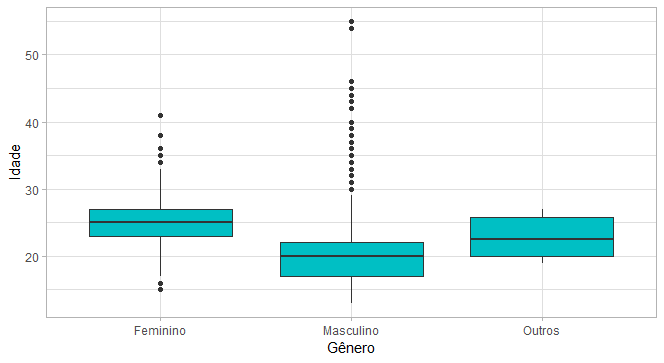
\includegraphics[width=0.45\textwidth]{idadegenero.png}
}
\subfigure[Mapa com os quantis]{ \label{subfig:grafico2}
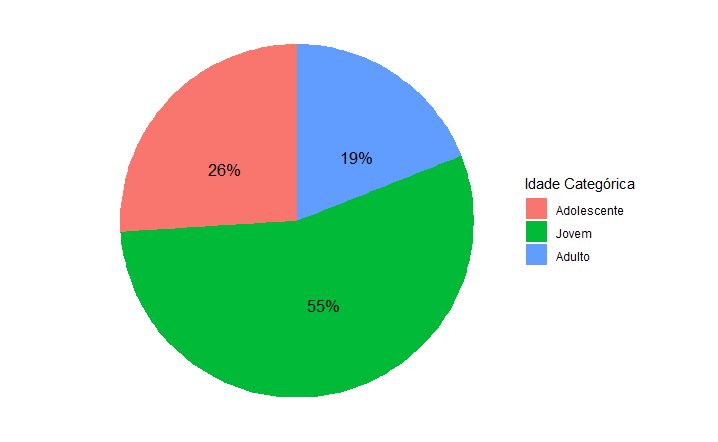
\includegraphics[width=0.45\textwidth]{idadecat.png}
}
\\
\vspace{1cm}
\subfigure[Mapa dos voluntarios por estados]{ \label{subfig:grafico3}
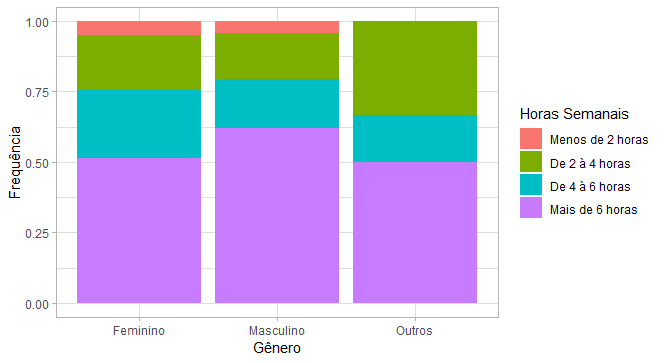
\includegraphics[width=0.45\textwidth]{generohoras.png}
}
\subfigure[Mapa com os quantis]{ \label{subfig:grafico4}
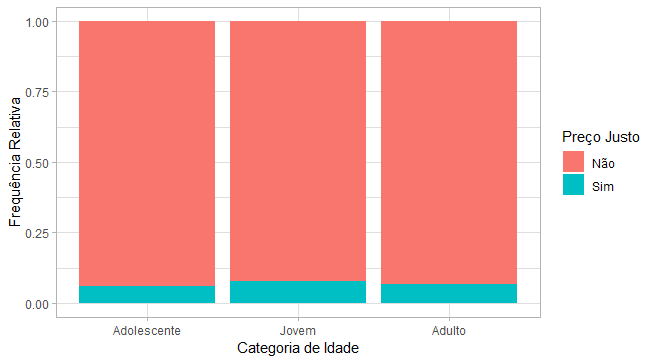
\includegraphics[width=0.45\textwidth]{IdadeJusto.png}
}
\\
\vspace{1cm}
\subfigure[Mapa com os quantis]{ \label{subfig:grafico5}
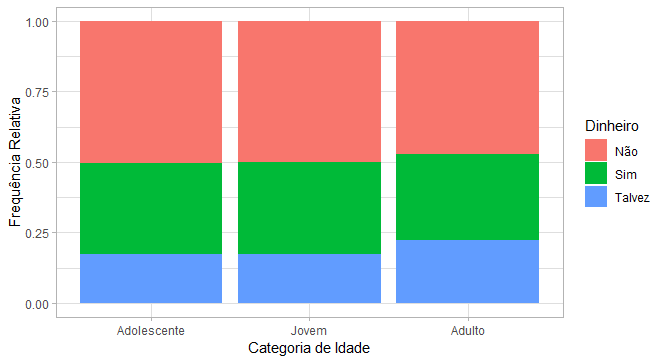
\includegraphics[width=0.45\textwidth]{IdadeDinheiro.png}
}
\subfigure[Mapa com os quantis]{ \label{subfig:grafico6}
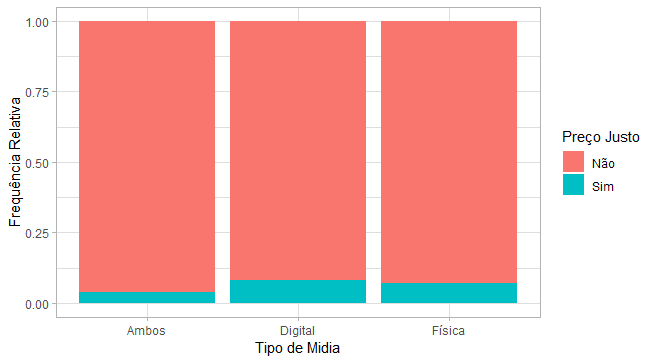
\includegraphics[width=0.4\textwidth]{Midiajusto.png}
}
\end{figure} 

\begin{figure}[t]
\centering
\subfigure[Generos]{ \label{subfig:grafico7}
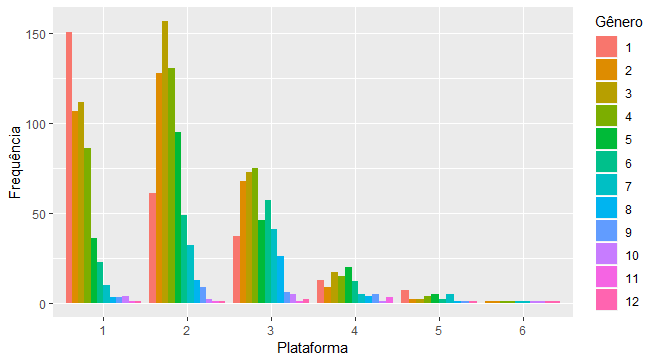
\includegraphics[width=0.7\textwidth]{platxgenero2.png}
}
\end{figure}

\begin{figure}[ht]
\centering
\subfigure[Tipo de Midia]{ \label{subfig:grafico8}
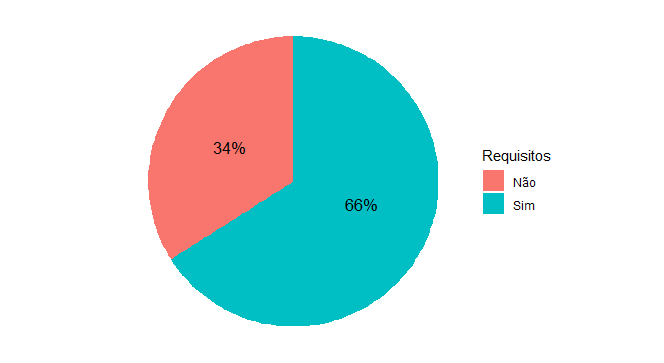
\includegraphics[width=0.45\textwidth]{pizzarequisitos.png}
}
\subfigure[Tipo de Midia]{ \label{subfig:grafico9}
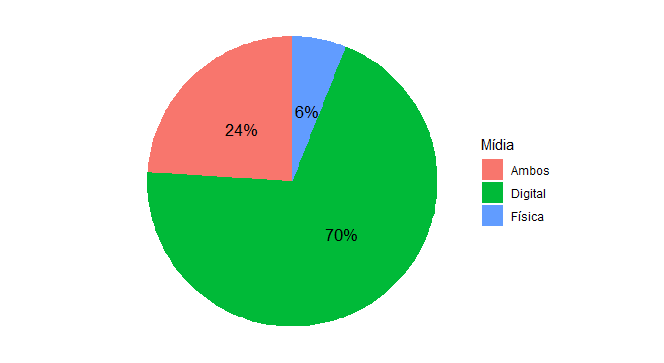
\includegraphics[width=0.45\textwidth]{pizzamidia.png}
}
\subfigure[Tipo de Midia]{ \label{subfig:grafico10}
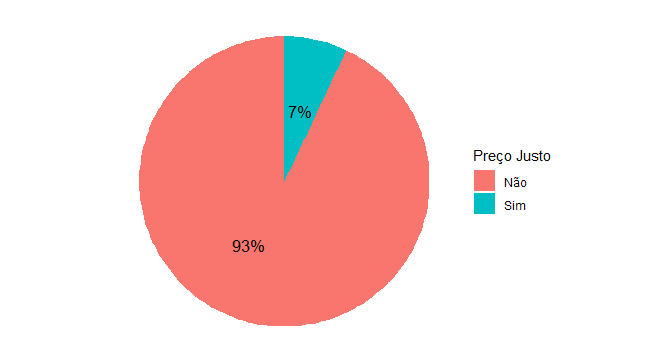
\includegraphics[width=0.45\textwidth]{pizzapreco.png}
}
\subfigure[Tipo de Midia]{ \label{subfig:grafico11}
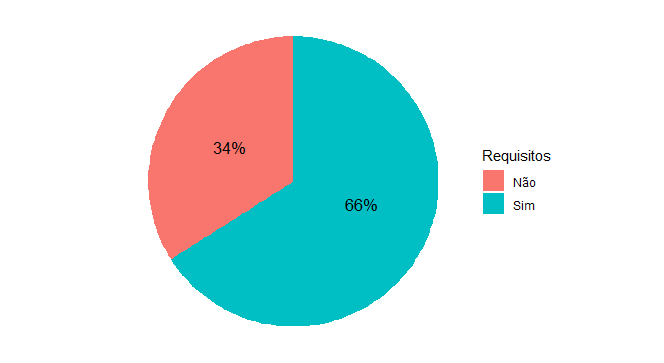
\includegraphics[width=0.45\textwidth]{pizzarequisitos.png}
}
\subfigure[Voce aca preço justo]{ \label{subfig:grafico12}
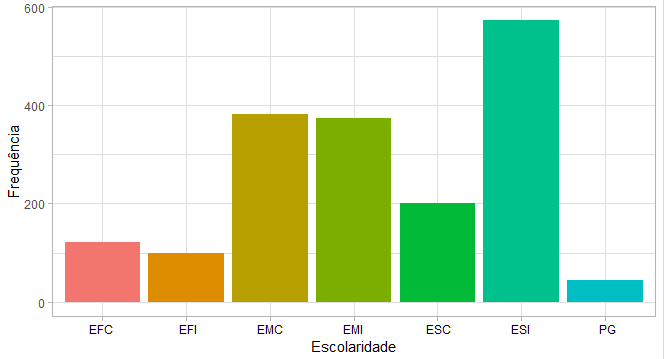
\includegraphics[width=0.6\textwidth]{barescoll.png}
}
\end{figure} 

\vspace{-1cm}

\begin{figure}[ht]
\centering
\subfigure[Generos]{ \label{subfig:grafico13}
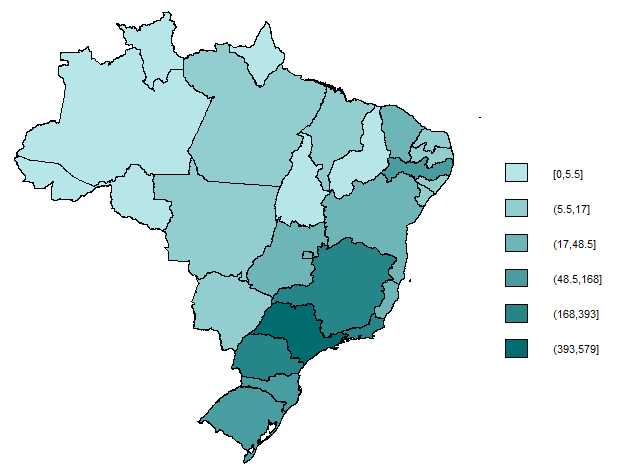
\includegraphics[width=0.7\textwidth]{mapa1.png}
}
\end{figure}

\end{document}